\documentclass[a4paper,oneside,12pt]{article}

\usepackage{custom}
\newcommand{\barg}{\si{\bar}\text{g}} 
\usepackage{setspace}
\usepackage{chemist}
\usepackage{fancyhdr} 
\usepackage{amsmath}
\fancyhf{}   
\fancyfoot[C]{\thepage}                     
\renewcommand\headrulewidth{0pt}
\pagestyle{fancy}

\begin{document}

\begin{titlepage} 
	\centering
	{\LARGE \textsc{Université Catholique de Louvain}}\\
	{\large \textsc{École Polytechnique de Louvain}}\\
	
	\vspace{1.3cm}
	
	\begin{center}
	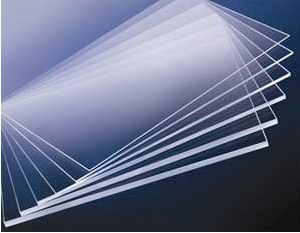
\includegraphics[scale=0.65]{Images/plexi.jpg}
	\end{center}
	
	\vspace{1.1cm}
	\hrulefill
	\\
	\vspace{0.9cm}
	{\huge \textbf{LMAPR1400}}\\
	\vspace{0.25cm}
	{\huge \textbf{Cinétique appliquée}} \\ 
	\vspace{0.7cm}
	{\huge \textbf{Cinétique de polymérisation du méthacrylate de méthyle}} \\
	\vspace{0.5cm}
	\hrulefill
	\\
	\vspace{0.9cm}
	
	\begin{center}
		\begin{tabular}{rl}
			
			\textsc{Dispas} David & (7189-12-00)\\
			\textsc{Paquet} Arnaud & (3668-13-00)\\
			
		\end{tabular}
	\end{center}
	
	\vfill
	
	\begin{center}
		
\includegraphics[scale=0.25]{Images/epl-logo.jpg}
	\end{center}
	
	\vspace{0.4cm}
	
	{\normalsize Année académique 2015 - 2016}\\
	
\end{titlepage}

\part{Applications du plexiglas dans la vie courante}

Le polyméthacrylate de méthyle (PMMA) est un polymère thermoplastique. Plus connu sous le nom de plexiglas, il possède des propriétés physiques très intéressantes.

Le PMMA est un matériau transparent. Ses propriétés optiques sont remarquables puisqu'il transmet jusqu'à $92\%$ de la lumière visible, soit plus que le verre. Il est parfaitement adapté pour remplacer le verre dans la fabrication de vitres, d'autant plus que le plexiglas est beaucoup plus léger que le verre et qu'il filtre les rayons ultraviolets. On l'utilise aussi pour les feux de voiture et dans certaines applications de redirection lumineuse.

Le plexiglas est également résistant. Il montre une importante rigidité, ainsi qu'une résistance à la corrosion, ce qui en fait le matériau idéal pour les vitres de grands aquariums.

Le PMMA est également fort présent dans la technologie médicale car il possède un haut degré de compatibilité avec le tissu humain.
Il est notamment utilisé dans la fabrication de lentilles intraoculaires, de prothèses dentaires ou encore dans la chirurgie orthopédique. 

On retrouve même la présence de plexiglas dans le domaine artistique.

\part{Evolution des concentrations}
La réaction que nous analysons est une polymérisation radicalaire. Elle peut donc être décomposée en les étapes suivantes:
\section{Amorçage}
L'amorceur utilisé est une molécule d'azobisisobutyronitrile (AIBN). 
\begin{equation}
	\ce{AIBN \underset{lent}{\xrightarrow{k_0}} N2 + 2A^{\bullet}}
\end{equation}	
La vitesse de décomposition de l'AIBN est très lente part rapport à la réaction suivante (\ref{2}). Seule une fraction f des radicaux créés est efficace pour réagir ensuite de la manière suivante:

\begin{equation}
\ce{A^{\bullet} + M \underset{rapide}{\xrightarrow{k_i}} R1^{\bullet}}
\label{2}
\end{equation}

où M est une molécule de méthacrylate de méthyle et $\ce{R_1^{\bullet}}$ est un radical en croissance. Nous pouvons utiliser l'hypothèse de quasi-stationnarité du radical (HQSR) $\frac{d[A^{\bullet}]}{dt}=0$ et ainsi obtenir que $2fk_{0}[AIBN]=k_{i}[A^{\bullet}][M]=r_i$.

\section{Propagation}
La chaîne devient de plus en plus grande en annexant des monomères. Pour une chaîne de longueur 1, nous avons :
\begin{equation}
\ce{R1^{\bullet} + M \xrightarrow{k_p} R2^{\bullet}}
\end{equation}
Nous pouvons généraliser cela à $\ce{R_j^{\bullet}}$, une chaîne en croissance composée d'un $A^{\bullet}$ auquel j monomères $M$ se sont ajoutés :
\begin{equation}
\ce{R_j^{\bullet} + M \xrightarrow{k_p} R_{j+1}^{\bullet}}
\end{equation}
Les constantes de vitesse $k_{p}$ de toutes les réactions de propagation sont considérés égales, ce qui n'est théoriquement valable que pour chaînes de longueur supérieure à quelques unités. Ceci est l'hypothèse d'équiréactivité de Flory.

\section{Terminaison}
Il existe deux types de terminaisons: la recombinaison et la dismutation. Travaillant à la température de 22,5$^{\circ}$C, nous négligerons ici la seconde qui ne se produit qu'à plus haute température. La réaction de recombinaison est la suivante:

\begin{equation}
\ce{R_{n}^{\bullet} + R_{m}^{\bullet} \xrightarrow{k_t} P_{n+m}}
\end{equation}
où $P_{j}$ est une molécule de PMMA de longueur j. Pour simplifier, nous ferons l'hypothèse que $k_{t}$ ne dépend pas de la longueur des chaînes.

\section{Transfert}
Nous disposons de plusieurs agents de transfert TrH pour lesquels nous connaissons les $C_{s}=\frac{k_{s}}{k_{p}}$. Ces derniers peuvent neutraliser une chaine et produire un radical qui pourra amorcer une nouvelle chaine:
\begin{equation}
\ce{R_{j}^{\bullet} + TrH \xrightarrow{k_s} R_{j}H + Tr^{\bullet}}
\label{6}
\end{equation}

\begin{equation}
\ce{Tr^{\bullet} + M \xrightarrow{k_i,tr} R_{1}^{\bullet}}
\end{equation}

Nous faisons l'hypothèse que $k_s$ est indépendant de la longueur des chaines.

\section{Calcul des lois de concentrations}
Le cas que nous considérons d'abord est très simplifié. Dans la partie suivante, nous prendrons en compte l'influence de phénomènes observés sur la cinétique du système. Le modèle sera ainsi plus réaliste. Mais dans un premier temps, nous considérons les constantes de vitesse comme indépendantes du temps. 

Nous choisissons également de ne pas prendre en compte la variation de concentration [AIBN]. La vitesse $r_i$ est donc considérée comme constante (étant donné que $r_i=2fk_0[AIBN]$).
Nous avons donc : 
$$[AIBN]=[AIBN]_{t=0}$$

% Commençons par calculer la concentration en AIBN. Puisque le composé n'apparait que dans la première équation, l'expression de sa vitesse de disparition est simplement: $-\frac{d[AIBN]}{dt}=k_{0}[AIBN]$. On trouve aisément la solution: $$[AIBN]=[AIBN]_{t=0}e^{-k_{0}t} $$.\\

De manière générale, la vitesse d'appairiton globale des chaînes $R^{\bullet}$ n'est autre que la somme des vitesses d'apparition $r_{m}$ de chaque chaîne $R_{m}$. Nous pouvons trouver que:

\begin{eqnarray*}
r_{1} &=& \frac{d[R_{1}^{\bullet}]}{dt}\\
      &=& r_{i}+k_{i,tr}[Tr^{\bullet}][M]-k_p[R_{1}^{\bullet}][M]-k_{t}[R_1^{\bullet}]\sum\limits_{j=1}^\infty[R_j^{\bullet}]-k_{s}[R_{1}^{\bullet}][TrH]
\end{eqnarray*}

\begin{eqnarray*}
r_{2} &=& \frac{d[R_{2}^{\bullet}]}{dt}\\
	&=& k_p[R_{1}^{\bullet}][M]-k_p[R_{2}^{\bullet}][M]-k_{t}[R_2^{\bullet}]\sum\limits_{j=1}^\infty[R_j^{\bullet}]-k_{s}[R_{2}^{\bullet}][TrH]
\end{eqnarray*}

\begin{eqnarray*}
r_{m} &=& \frac{d[R_{m}^{\bullet}]}{dt}\\
      &=& k_p[R_{m-1}^{\bullet}][M]-k_p[R_{m}^{\bullet}][M]-k_{t}[R_m^{\bullet}]\sum\limits_{j=1}^\infty[R_j^{\bullet}]-k_{s}[R_{m}^{\bullet}][TrH]
\end{eqnarray*}

Par conséquent:

$$\sum\limits_{m=1}^\infty r_{m}=r_i+ k_{i,tr}[Tr^{\bullet}][M] -k_{t}\sum\limits_{m=1}^\infty [R_m^{\bullet}] \sum\limits_{j=1}^\infty[R_j^{\bullet}]-k_{s}\sum\limits_{m=1}^\infty[R_{m}^{\bullet}][TrH]$$
Et en remarquant que :
$$\sum\limits_{j=1}^\infty[R_j^{\bullet}] = [R^{\bullet}]$$
Nous pouvons écrire :
$$\sum\limits_{m=1}^\infty r_{m}=r_i+ k_{i,tr}[Tr^{\bullet}][M] -k_{t}[R^{\bullet}]^2-k_{s}\sum\limits_{m=1}^\infty[R_{m}^{\bullet}][TrH]$$
De plus, l'HQSR appliquée sur $Tr^{\bullet}$ nous donne :
$$\frac{d[Tr^{\bullet}]}{dt}=0=k_{i,tr}[Tr^{\bullet}][M]-k_{s}\sum\limits_{m=1}^\infty[R_{m}^{\bullet}][TrH]$$
Les termes s'annulent et nous pouvons donc simplifier notre expression :
$$\sum\limits_{m=1}^\infty r_{m}=r_i-k_{t}[R^{\bullet}]^2$$
Finalement, en tenant compte que l'HQSR des radicaux $R^{\bullet}$ :
$$\sum\limits_{m=1}^\infty r_{m}=0$$
Nous obtenons :
$$r_i = k_{t}[R^{\bullet}]^2$$
$$[R^{\bullet}] = (\frac{r_i}{k_t})^{\frac{1}{2}}
		        = (\frac{2fk_0[AIBN]}{k_t})^{\frac{1}{2}}$$
		        
La concentration en $R^{\bullet}$ est constante !\\

Calculons maintenant la concentration en agent de transfert. Ce composé n'apparait que dans une réaction (\ref{6}). La vitesse de disparition de $TrH$ vaut : 
$$r_{tr}=-\frac{d[TrH]}{dt}=k_s[R^{\bullet}][TrH]$$
Il s'en suit que :
$$ln([TrH])=-k_s[R^{\bullet}]\int_{0}^t dt'$$
Ce qui donne après intégration :
$$[TrH]=e^{-k_s[R^{\bullet}]t}[TrH]_{t=0}$$

%$$ln[TrH]=\frac{2k_{s}}{k_0}[R^{\bullet}]_{t=0}(e^{-k_{0}t/2} - 1)+c=\frac{2k_{s}}{k_0}([R^{\bullet}]-[R^{\bullet}]_{t=0})+c$$
%$$[TrH]=e^{\frac{2k_{s}}{k_0}([R^{\bullet}]-[R^{\bullet}]_{t=0})}[TrH]_{t=0}$$

Passons maintenant à la concentration en monomères M. La vitesse de disparition de M est :
$$r_M=-\frac{d[M]}{dt}=r_{i}+k_{i,tr}[Tr^{\bullet}][M]+k_{p}[R^{\bullet}][M]$$ 
En faisant l'hypothèse des chaînes longues, nous pouvons considérer que les deux vitesses d'amorçage sont négligeables par rapport à celle de propagation. On retrouve donc :
$$-\frac{d[M]}{dt}\cong k_{p}[R^{\bullet}][M]$$ 
Cela se résout exactement de la même manière que pour l'agent de transfert :
$$[M]=e^{-k_p[R^{\bullet}]t}[M]_{t=0}$$

%$$[M]=e^{\frac{2k_{p}}{k_0}([R^{\bullet}]-[R^{\bullet}]_{t=0})}[M]_{t=0}$$

%Calculons finalement la concentration en PPMA. La vitesse d'apparition du PMMA est donnée par :
%$$\frac{d[P]}{dt}=k_{t}[R^{\bullet}]^2+k_{s}[R^{\bullet}][TrH]$$
%On obtient alors la fonction à intégrer pour trouver [P]. Si nous négligeons l'impact de l'agent de transfert $TrH$, on voit de manière immédiate que :
%$$[P]=r_i t$$

%En tenant compte de l'agent de transfert :
%En développant et mettant les $[R^{\bullet}]_{t=0}$ en évidence, on obtient :
%$$[P]=\int_{0}^t ([R^{\bullet}]^{2}_{t=0}k_te^{-k_0t'}+k_s[R^{\bullet}]_{t=0}e^{\frac{-k_0t'}{2}}e^{2\frac{k_s}{k_0}[R^{\bullet}]_{t=0}(e^{-k_0t'/2}-1)})dt'$$

%Le résultat de cette intégrale est:
%$$[P]=-\frac{k_t[R^{\bullet}]_{t=0}^2e^{-k_0t}}{k_0}+\frac{k_t[R^{\bullet}]_{t=0}^2}{k_0}+k_s[R^{\bullet}]_{t=0}e^{\frac{k_s[R^{\bullet}]_{t=0}(e^{\frac{-k_0t}{2}}-1)}{k_0}-\frac{k_0t}{2}}-k_s[R^{\bullet}]_{t=0}$$
%$$[P]=2f[AIBN]_{t=0}(1-e^{-k_0t})+k_s[R^{\bullet}]_{t=0}(e^{\frac{k_s[R^{\bullet}]_{t=0}(e^{\frac{-k_0t}{2}}-1)}{k_0}-\frac{k_0t}{2}}-1)$$


\section{Degré de polymérisation}
Soit $\alpha$ la probabilité d'allongement d'une chaine radicalaire en croissance par propagation : 
$$\alpha=\frac{k_p[R^{\bullet}][M]}{k_p[R^{\bullet}][M]+k_s[R^{\bullet}][TrH]+k_t[R^{\bullet}]^2}$$

On obtient le degré de polymérisation moyen instantané en nombre (DPn) ou en poids (DPw) comme des fonctions dépendant du temps:
$$DPn=\frac{2}{1-\alpha}$$
$$DPw=\frac{2+\alpha}{1-\alpha}$$

\section{Graphes}
Les résultats suivants sont obtenus en négligeant la réaction de transfert et avec le set de données suivant:

%INSERER GRAPHES!!!

\part{Influence des différents effets observés}

Ajoutons maintenant les différents phénomènes pouvant altérer la cinétique des réactions.\\

\section{L'effet Trommsdorff} 
Egalement appelé effet "gel" ou d'auto-accélération, il est responsable d'une baisse du $k_t$ corrélée de manière exponentielle à la concentration en monomères. En effet, au fil de la réaction, les chaines créées deviennent de plus en plus longues, s'emmêlent et perdent leur diffusivité par rapport au monomères. Les terminaisons, nécessitant deux radicaux, deviennent donc plus difficiles et la propagation gagne en importance. Le DPn augmente donc.\\

Des valeurs expérimentales de $k_t$ en fonction de la fraction convertie en monomères nous ont été données. Nous avons approximé ces valeurs par une droite. Comme $k_t$ varie maintenant avec le temps, nous devons adapter [M] qui doit maintenant être égal à:
$$[M]=e^{-k_pr_i^{\frac{1}{2}}\int_0^t k_t^{\frac{-1}{2}}dt'}[M]_{t=0}$$
Connaissant $k_t$ en fonction de [M], nous devons alors résoudre un système de deux équations à 2 inconnues ce que nous pouvons faire numériquement. Voilà les résultats:.................\\

\section{L'effet de vitrification}
L'effet de vitrification: nous sommes à une température bien en dessous de celle de vitrification du PMMA. Par conséquent, le système passe progressivement vers une transition vitreuse et la mobilité des monomères en est diminuée: $k_p$ diminue donc aussi jusqu'à tomber à 0. Système à un état trop visqueux/solide pour que la réaction puisse continuer. Pour une température entre 20 et 50$^{\circ}$C, le taux de conversion va de 60 à 90 $\%$ \footnote{https://books.google.be/books?
id=0jGnykE4PuEC$\&$pg=PA41$\&$lpg=PA41$\&$dq=polym$\%$C3$\%$A9risation+radicalaire+vitrification$\&$source=bl$\&$ots=4dQord5Zcu$\&$sig=WaEfwFHcsy8daffRxj49SCK1XDY$\&$hl=fr$\&$sa=X$\&$ved=0ahUKEwiz8aWfjeDJAhWG1RQKHan2BrEQ6AEIHzAA$\#$v=onepage$\&$q=polym
$\%$C3$\%$A9risation$\%$20radicalaire$\%$20vitrification$\&$f=false}.
Pour que cet effet disparaisse, on devrait augmenter la température de manière suffisante.\\
Puisque des données expérimentales nous sont fournies, nous pouvons déterminer l'évolution des constantes $k_t$ et $k_p$.\\

\section{L'effet de l'agent de transfert}
L'ajout d'un agent de transfert à tout d'abord l'effet majeur de diminuer globalement le degré de polymérisation. En effet, il réagit avec les chaines $R^{\bullet}$ et stoppe leur croissance, tout en créant des nouvelle chaine $R_1^{\bullet}$. On voit également grâce à nos calculs que la vitesse de production de polymères morts est diminuée, avec un impact plus grand pour un agent de transfert dont le $C_s$ est plus grand.


\part{Epuisement de l'amorceur}

\part{Effets de la température}

\end{document}
